%==============================================================================
%  Trabalho Final — Teoria da Informação (TIP7266 / PGETI-UFC) — 2026.1
%  Information-Theoretic Characterization of Aging Information and Noise
%  in On-Chip Slack Sensors for Silicon Lifecycle Management
%
%  Build:  pdflatex main && bibtex main && pdflatex main && pdflatex main
%  (or simply: latexmk -pdf main.tex)
%
%  Document class: 'article' is used for maximum portability. To submit in
%  IEEE format, replace the \documentclass line below with:
%      \documentclass[conference]{IEEEtran}
%  and remove the geometry/abstract tweaks that IEEEtran already provides.
%==============================================================================
\documentclass[11pt,a4paper]{article}

\usepackage[utf8]{inputenc}
\usepackage[T1]{fontenc}
\usepackage[english]{babel}
\usepackage[margin=1in]{geometry}

% --- math ---
\usepackage{amsmath,amssymb,amsfonts}
\usepackage{bm}

% --- tables / figures ---
\usepackage{booktabs}
\usepackage{graphicx}
\graphicspath{{figures/}}
\usepackage{multirow}

% --- references / links ---
\usepackage[numbers,sort&compress]{natbib}
\usepackage[hidelinks]{hyperref}
\usepackage{cleveref}

% --- project-wide notation macros (single source of truth) ---
%==============================================================================
%  notation.tex — project-wide symbols and operators.
%  Keeping these in one place guarantees the slack/PVT model is written
%  identically in every section.
%==============================================================================

% random variables
\newcommand{\slk}{S}                 % slack reading (sensor output)
\newcommand{\Tdie}{T}                % die temperature
\newcommand{\Vcore}{V}               % core voltage
\newcommand{\tm}{t}                  % time (\time is a TeX primitive)

% model components
\newcommand{\saged}{S_{\mathrm{aged}}}      % permanent aging term
\newcommand{\dpvt}{\Delta_{\mathrm{PVT}}}   % reversible PVT term
\newcommand{\eq}{\varepsilon_q}             % quantization noise
\newcommand{\scorr}{S_{\mathrm{corr}}}      % PVT-corrected residual

% information-theoretic operators
\newcommand{\Ent}[1]{H\!\left(#1\right)}                 % entropy
\newcommand{\MI}[2]{I\!\left(#1 ; #2\right)}             % mutual information
\newcommand{\KL}[2]{D_{\mathrm{KL}}\!\left(#1 \,\|\, #2\right)}  % KL divergence
\newcommand{\neff}{n_{\mathrm{eff}}}                     % effective sample size
\newcommand{\tauint}{\tau_{\mathrm{int}}}                % integrated autocorr. time
\newcommand{\Hb}{H_2}                                    % binary entropy function
\newcommand{\Cbsc}{C_{\mathrm{BSC}}}                     % BSC capacity

% complexity, estimation and ICA operators
\newcommand{\Kolm}[1]{K\!\left(#1\right)}                % Kolmogorov complexity
\newcommand{\Neg}[1]{N_G\!\left(#1\right)}               % negentropy
\newcommand{\FI}{\mathcal{I}_F}                          % Fisher information

% Wiener-process degradation / Kalman filtering operators
\newcommand{\Xlat}{X}                    % latent (denoised) aging level
\newcommand{\IG}[2]{\mathrm{IG}\!\left(#1,#2\right)}     % Inverse Gaussian(mean,shape)

% the inherited signal model, written once
\newcommand{\signalmodel}{%
  \slk(\tm) = \saged(\tm) - \dpvt(\Tdie,\Vcore) + \eq
}


% --- numbers produced by the analysis pipeline (auto-generated; see 05_Execution_Plan.md) ---
%==============================================================================
%  generated/values.tex
%  Scalar results injected from the analysis pipeline. Edit via the analysis
%  scripts, NOT by hand, so the paper and the data never drift apart.
%  (See 05_Execution_Plan.md, "Pipeline contract".)
%
%  Values below were computed from Tentative_1_20260524_203756.csv.
%  All values are filled by the analysis scripts (tier1_pipeline.py,
%  kl_benches.py, ica_separation.py). Re-run them to regenerate.
%==============================================================================

% --- dataset (computed) ---
\newcommand{\valDurationHours}{214.6}
\newcommand{\valRawSamples}{772{,}484}
\newcommand{\valPostSoakSamples}{768{,}884}
\newcommand{\valDropouts}{5}
\newcommand{\valDutTempMean}{125.1}
\newcommand{\valDutVoltMean}{1.400}
\newcommand{\valSlackMean}{278.5}
\newcommand{\valSlackStd}{3.03}
\newcommand{\valSlackLevels}{27}
\newcommand{\valSlackRange}{267\text{--}300}

% --- second-order relationships (computed) ---
\newcommand{\valCorrST}{-0.859}
\newcommand{\valCorrSV}{+0.213}
\newcommand{\valCorrSt}{-0.348}
\newcommand{\valSlopeRaw}{-0.0171}
\newcommand{\valRsqLinear}{0.738}

% --- entropy (computed, discrete plug-in) ---
\newcommand{\valHs}{3.43}

% --- prior-work anchors (external published numbers from the
%     thermal-fidelity paper; intentionally NOT recomputed by this
%     pipeline -- there is no raw log for the bang-bang regime) ---
\newcommand{\valRsqBangBang}{0.921}
\newcommand{\valRsqPid}{0.592}
\newcommand{\valSigmaBangBang}{3.29}    % deg C
\newcommand{\valSigmaPid}{0.40}         % deg C
\newcommand{\valResidBangBang}{0.90}    % counts
\newcommand{\valResidPid}{0.73}         % counts
\newcommand{\valLSBps}{19.85}           % ps per slack count

% --- Tier-1 information measures (tier1_pipeline.py) ---
\newcommand{\valMIst}{1.087}
\newcommand{\valMIsv}{0.113}
\newcommand{\valMIstv}{1.132}
\newcommand{\valInfoFraction}{0.330}
\newcommand{\valHscondTV}{2.30}
\newcommand{\valKSGstv}{1.221}
\newcommand{\valMIciLo}{1.091}
\newcommand{\valMIciHi}{1.176}
\newcommand{\valMIlinEquiv}{0.967}
\newcommand{\valMIexcessPct}{17}
\newcommand{\valMIexcessPctBinned}{17}
\newcommand{\valMIexcessPctKSG}{26}
\newcommand{\valMIexcessCiLoBinned}{13}
\newcommand{\valMIexcessCiHiBinned}{22}
\newcommand{\valMIexcessCiLoKSG}{20}
\newcommand{\valMIexcessCiHiKSG}{32}
\newcommand{\valMIbins}{16}
\newcommand{\valMIbinSensLo}{1.111}
\newcommand{\valMIbinSensHi}{1.171}
\newcommand{\valKSGciLo}{1.156}
\newcommand{\valKSGciHi}{1.275}
\newcommand{\valMIexcessFloorAdjBits}{0.10}
\newcommand{\valMIexcessFloorAdjPct}{10}
\newcommand{\valRsqDetrended}{0.640}
\newcommand{\valMIlinEquivDetrended}{0.736}
\newcommand{\valMIdtBinned}{0.596}
\newcommand{\valMIdtCiLo}{0.582}
\newcommand{\valMIdtCiHi}{0.632}
\newcommand{\valMIexcessPctDetrended}{-19}
\newcommand{\valMIdtKSG}{0.656}
\newcommand{\valMIdtKsgCiLo}{0.622}
\newcommand{\valMIdtKsgCiHi}{0.735}
\newcommand{\valMIexcessPctDetrKSG}{-11}
\newcommand{\valMInullFloor}{0.097}
\newcommand{\valMInullMean}{0.069}
\newcommand{\valMIfloorRatio}{12}
\newcommand{\valResidMI}{0.046}
\newcommand{\valPreMIrev}{0.656}
\newcommand{\valResidMIlin}{0.046}
\newcommand{\valResidMInl}{0.024}
\newcommand{\valResidSigmaLin}{0.84}
\newcommand{\valResidSigmaNL}{0.84}
\newcommand{\valCorrModel}{linear}
\newcommand{\valMIreductionPct}{93}
\newcommand{\valCorrStRaw}{-0.35}
\newcommand{\valCorrStCorr}{-0.73}
\newcommand{\valNeff}{1{,}224}
\newcommand{\valTauInt}{314}
\newcommand{\valAgingSlope}{-18.3}
\newcommand{\valSigSignal}{1.29}
\newcommand{\valSigNoise}{0.84}
\newcommand{\valSNR}{2.36}
\newcommand{\valCapacityBits}{0.87}
\newcommand{\valCapacityStates}{1.8}
\newcommand{\valCRLBsd}{0.39}
\newcommand{\valMinDetectRate}{1.2}
\newcommand{\valMinObsTime}{34}
\newcommand{\valBSCwindow}{24}
\newcommand{\valBSCp}{0.001}
\newcommand{\valBSCcap}{0.99}
% --- Bayesian posterior on the aging slope (tier1_pipeline.py) ---
\newcommand{\valBayesSlope}{-18.2}
\newcommand{\valBayesSlopeLo}{-19.2}
\newcommand{\valBayesSlopeHi}{-17.2}
\newcommand{\valBayesPaging}{100.00}
\newcommand{\valBayesMotLo}{33}
\newcommand{\valBayesMotHi}{36}
% --- KL / Jensen-Shannon between benches (kl_benches.py) ---
\newcommand{\valSlackStdSBCCI}{3.23}
\newcommand{\valSlackStdPID}{1.46}
\newcommand{\valTstdSBCCI}{2.64}
\newcommand{\valTstdPID}{1.25}
\newcommand{\valKLsp}{1.94}
\newcommand{\valKLps}{1.01}
\newcommand{\valJSbench}{0.279}
\newcommand{\valKLgauss}{1.67}

% --- ICA blind source separation (ica_separation.py) ---
\newcommand{\valICAagingScorr}{0.834}
\newcommand{\valICAagingVarExpl}{70}
\newcommand{\valICAagingTime}{-0.575}
\newcommand{\valICAthermalT}{0.688}
\newcommand{\valICAkurtAging}{+5.82}
\newcommand{\valICAkurtThermal}{+29.91}
\newcommand{\valICAresidMI}{0.571}
\newcommand{\valICAverdict}{recovers}

% --- Wiener/Kalman aging-trajectory + RUL extension (kalman_rul.py) ---
\newcommand{\valWienerSigmaB}{0.403}
\newcommand{\valWienerQRate}{1.0\times10^{-10}}
\newcommand{\valWienerRateEnd}{-15.9}
\newcommand{\valWienerLevelSDstart}{0.214}
\newcommand{\valWienerLevelSDend}{0.218}
\newcommand{\valRULmeanNoise}{52.9}
\newcommand{\valRULmedianNoise}{8.0}
\newcommand{\valRULmeanSignal}{81.3}
\newcommand{\valRULmedianSignal}{17.5}
\newcommand{\valDnoise}{0.84}
\newcommand{\valDsignal}{1.29}
\newcommand{\valNBlocks}{1{,}224}


\title{\textbf{Information-Theoretic Characterization of Aging Information and
Noise in On-Chip Slack Sensors for Silicon Lifecycle Management}}

\author{%
  Danilo Alencar\\
  \small Programa de P\'os-Gradua\c{c}\~ao em Engenharia de Teleinform\'atica (PGETI)\\
  \small Universidade Federal do Cear\'a\\
  \small Disciplina: Teoria da Informa\c{c}\~ao (TIP7266) --- Trabalho Final, 2026.1
}
\date{\today}

\begin{document}
\maketitle

%==============================================================================
\begin{abstract}
On-chip slack sensors used in Silicon Lifecycle Management (SLM) report a
quantity that mixes a permanent, slowly-drifting aging component with a
reversible component driven by process, voltage and temperature (PVT). Prior
work quantifies this contamination with the coefficient of determination
($R^2$) of a linear regression of slack on temperature and voltage---a measure
that captures only linear dependence and yields no transferable unit. This work
places an \emph{information-theoretic measurement layer} on top of an existing
low-cost accelerated-aging burn-in platform and its synchronized
\mbox{(slack, $\Tdie$, $\Vcore$, time)} logs. Treating the sensor as a noisy
communication channel, we (i)~replace $R^2$ with the mutual information
$\MI{\slk}{\Tdie,\Vcore}$ as the correct, non-linear measure of environmental
contamination; (ii)~quantify, in bits, how much uncertainty PVT logging removes
via $\Ent{\slk}-\Ent{\slk\mid\Tdie,\Vcore}$; (iii)~estimate the sensor's
effective resolving power through a channel-capacity heuristic and a Binary
Symmetric Channel model of the aging-alarm decision; (iv)~derive a
noise-limited detectability bound for remaining-useful-life (RUL) estimation,
via both a Cram\'er--Rao/Bayesian point estimate and a sequential Wiener-process/
Kalman-filter treatment that yields a denoised aging trajectory with credible
bands and a full, closed-form Inverse-Gaussian RUL distribution. We further
apply MDL model selection and ICA-based blind source separation to the same
data, and a KL/Jensen--Shannon comparison of two validation benches. On a
\valDurationHours~h PID-controlled campaign (\valPostSoakSamples{} post-soak
samples; effective sample size $\neff=\valNeff$) we measure
$\Ent{\slk}=\valHs$~bits and $\MI{\slk}{\Tdie,\Vcore}=\valMIstv$~bits
(KSG cross-check \valKSGstv~bits). This measured dependence exceeds the
Gaussian-equivalent MI of the prior work's linear fit
($R^2=\valRsqLinear\Rightarrow\valMIlinEquiv$~bits) by \valMIexcessPct\,\%,
directly evidencing the non-linear environmental coupling that $R^2$ cannot
capture. The contribution is a correct, transferable noise metric for SLM
sensors and a principled, optimizable definition of burn-in quality as the
minimization of environment--sensor mutual information.
\end{abstract}

\noindent\textbf{Keywords:} information theory; mutual information; entropy;
channel capacity; silicon lifecycle management; aging sensor; slack;
burn-in; remaining useful life.


%==============================================================================
\section{Introduction}
\label{sec:intro}

% --- maps to 01_Project_Overview.md §1, §2 ---

\subsection{Motivation and point of departure}
Integrated circuits degrade. Bias-temperature instability (BTI/NBTI), hot-carrier
injection and related mechanisms slow critical paths over a device's lifetime,
and SLM aims to monitor that degradation in-field to enable adaptive voltage
scaling and remaining-useful-life (RUL) prediction. This project builds on three
correlated prior efforts: an auto-tuning on-chip slack sensor
\cite{nogueira_sensor}, a thermal-control fidelity study comparing bang-bang and
PID burn-in ovens on the same device and sensor \cite{alencar_fidelity}, and a
low-cost automated burn-in platform \cite{alencarfilho_tcc}. Across all three, a
single fact recurs: the slack a sensor reports is a \emph{mixture} of a
permanent aging term and a reversible PVT term,
\begin{equation}
  \signalmodel ,
  \label{eq:model}
\end{equation}
where $\eq$ is quantization noise bounded by the sensor LSB
(\valLSBps~ps per count).

\subsection{The gap}
The prior work measures the reversible contamination with the linear $R^2$ of
slack regressed on $\Tdie$ and $\Vcore$ (e.g.\ \valRsqBangBang{} under bang-bang
vs.\ \valRsqPid{} under PID control). This has two limitations central to this
physical domain: it captures \emph{only linear} dependence, although BTI is
super-linear in $\Vcore$ and the Arrhenius acceleration is exponential in
inverse temperature; and it yields \emph{no transferable unit}---``variance
explained'' does not answer how many aging states the sensor resolves, how early
a trend is detectable, or how much aging information a given bench preserves.
Information theory answers all three in one currency: \textbf{bits}.

\subsection{Contribution}
We add an analytical measurement layer---no new silicon, sensor, or oven---that
re-expresses noise, correction and recoverability in the language of entropy,
mutual information and channel capacity. Concretely:
\begin{enumerate}
  \item $\MI{\slk}{\Tdie,\Vcore}$ replaces $R^2$ as a non-linear contamination
        measure (\cref{sec:results});
  \item an entropy account of PVT correction quantifies, in bits, the
        uncertainty each auxiliary channel removes;
  \item a capacity estimate and a BSC alarm model convert measured noise into
        resolvable aging states and alarm reliability;
  \item a Cram\'er--Rao/Bayesian detectability bound states the earliest
        detectable aging trend given the noise floor, complemented by a
        Wiener-process/Kalman-filter treatment that turns the same problem
        into a continuously-updated, denoised aging trajectory and a
        closed-form Inverse-Gaussian RUL \emph{distribution}
        (\cref{sec:res-wiener}).
\end{enumerate}
We additionally exercise source coding, Kolmogorov/MDL model selection and
ICA-based blind separation on the same logs, so that the project spans the full
syllabus of the course (\cref{sec:methodology} and the topic mapping).

\subsection{Scope and honesty}
The primary dataset is a single \valDurationHours~h PID campaign on one device;
it is long enough to expose a measurable aging drift but cannot, alone,
cross-validate a permanent-aging trajectory across devices. RUL results are thus
framed as a \emph{methodology and a detectability bound}. Mutual-information
estimation on strongly autocorrelated series is bias-prone; we report everything
on an effective sample size $\neff$ with block-bootstrap intervals.

%==============================================================================
\section{Background and Related Work}
\label{sec:background}

% --- maps to 01_Project_Overview.md §1; artigos/ ---

\subsection{The on-chip slack sensor}
The auto-tuning aging sensor \cite{nogueira_sensor} measures critical-path
timing slack on a Xilinx Artix-7 FPGA using a dynamically phase-shifted clock,
reporting one slack count per \valLSBps~ps phase increment, and tracks delay
degradation under burn-in, temperature and voltage stress.

\subsection{Thermal-control fidelity}
The thermal-fidelity study \cite{alencar_fidelity} compares a thermostatic
bang-bang oven against a closed-loop PID oven on the \emph{same} device and
sensor, showing that the burn-in thermal architecture changes both the delivered
acceleration factor and the reversible environmental noise on the sensor output.
It reports a steady-state thermal standard deviation of $\sigma=\valSigmaPid$~$^\circ$C
(PID) vs.\ $\valSigmaBangBang$~$^\circ$C (bang-bang), residual slack noise of
$\valResidPid$ vs.\ $\valResidBangBang$ counts, and a linear variance-explained of
$\valRsqPid$ vs.\ $\valRsqBangBang$. These are the numbers this work re-expresses
in information-theoretic terms.

\subsection{The automated burn-in platform}
The platform \cite{alencarfilho_tcc} delivers PID-controlled, multi-threaded
acquisition logging slack with synchronized temperature and voltage at 1~Hz. The
dataset analyzed here (\cref{sec:dataset}) is one such log.

\subsection{Why information theory}
\Cref{eq:model} is, in information terms, a noisy channel: the transmitter is the
latent degradation state, the channel adds reversible PVT fluctuation and
quantization noise, and the receiver estimates the slow aging trajectory. This
framing makes entropy, mutual information and capacity the natural figures of
merit and motivates the methodology of \cref{sec:methodology}.

\subsection{Why $R^2$ is structurally blind to the physics}
\label{sec:background-r2}
The deeper reason $R^2$ understates environmental coupling is not incidental to
this dataset---it is structural. $R^2$ is a monotone function of the Pearson
correlation/covariance between $\slk$ and its linear fit on $(\Tdie,\Vcore)$, and
$\mathrm{Cov}(X,Y)=0$ characterizes only the \emph{absence of linear}
association: independence implies zero covariance, but the converse is false in
general (a textbook example is $Y=X^2$ for symmetric $X$, where $\mathrm{Cov}=0$
yet $Y$ is a deterministic, fully dependent function of $X$). Consequently any
regression-$R^2$ metric can read as ``mostly independent'' a variable that is, in
fact, entirely determined by the inputs through a non-linear map---precisely the
situation here, since BTI aging acceleration is super-linear in $\Vcore$ and the
Arrhenius rate is exponential in $1/\Tdie$. Mutual information
(\cref{sec:th-mi}) is built from the full joint distribution rather than a
second-moment summary, so $\MI{\slk}{\Tdie,\Vcore}=0$ if and only if $\slk$ and
$(\Tdie,\Vcore)$ are independent, with no linearity assumption---closing exactly
the gap this section identifies.

%==============================================================================
\section{Information-Theoretic Framework}
\label{sec:theory}

% --- maps to 03_Course_Topic_Mapping.md; defines every course tool used ---
% This section is where the course content is formally introduced. Each
% subsection states the definition, its key properties/theorem AND its role
% in the sensor problem, so the link between syllabus and application is
% explicit (rubric item 03).

\subsection{Self-information and entropy}
\label{sec:th-entropy}
For a discrete source with alphabet $\{s_k\}$ and probabilities $p_k=P(\slk=s_k)$,
the \emph{self-information} of an outcome is $I(s_k)=-\log_2 p_k$: rare outcomes
are more surprising and carry more information, and independence makes
self-information additive, $I(s_ks_j)=I(s_k)+I(s_j)$ for independent $s_k,s_j$---the
property that forces the logarithm in the definition, since only $\log$ turns a
product of probabilities into a sum. \textbf{Entropy} is the expected
self-information,
\begin{equation}
  \Ent{\slk} = -\sum_k p_k\log_2 p_k = E\{I(\slk)\},
  \label{eq:entropy}
\end{equation}
the total uncertainty of the sensor reading, bounded by $0\le\Ent{\slk}\le\log_2 K$
($K$ = number of slack levels): zero when one level is certain, maximal when all
$K$ levels are equiprobable. The conditional entropy
$\Ent{\slk\mid\Tdie,\Vcore}$ is the residual uncertainty once the environment is
known, and the chain rule $\Ent{\slk,\Tdie,\Vcore}=\Ent{\Tdie,\Vcore}+\Ent{\slk\mid\Tdie,\Vcore}$
decomposes total uncertainty into an environmental part and a residual part---the
gap between $\Ent{\slk}$ and $\Ent{\slk\mid\Tdie,\Vcore}$ \emph{is} the
environmental information, formalized as mutual information next.

\subsection{Kullback--Leibler divergence and mutual information}
\label{sec:th-mi}
For two distributions $p,g$ over the same alphabet,
\begin{equation}
  \KL{p}{g} = \sum_x p(x)\log_2\frac{p(x)}{g(x)} = E_p\!\left\{\log_2\frac{p(x)}{g(x)}\right\}
  \label{eq:kl}
\end{equation}
measures the cost, in bits, of assuming $g$ when the true law is $p$.
$\KL{p}{g}\ge0$ with equality iff $p=g$: writing $-\log_2(\cdot)$, a convex
function, Jensen's inequality gives
$\KL{p}{g}=E_p\{-\log_2\frac{g(x)}{p(x)}\}\ge-\log_2 E_p\{\frac{g(x)}{p(x)}\}=-\log_2\sum_x g(x)=0$.
$D_{\mathrm{KL}}$ is \emph{not symmetric} and does not satisfy the triangle
inequality, so it is not a metric---exactly the asymmetry exploited in
\cref{sec:res-kl} to read $\KL{p_{\text{SBCCI}}}{p_{\text{PID}}}$ as ``the cost of
describing the noisy bench with the tight reference'' and not the reverse.
\textbf{Mutual information} is the KL divergence between the joint law and the
product of marginals,
\begin{equation}
  \MI{\slk}{\Tdie,\Vcore} = \KL{p(\slk,\Tdie,\Vcore)}{p(\slk)p(\Tdie,\Vcore)}
  = \Ent{\slk}-\Ent{\slk\mid\Tdie,\Vcore} \ge 0,
  \label{eq:mi}
\end{equation}
zero iff $\slk\perp(\Tdie,\Vcore)$, and, via the entropy Venn diagram (the union
of the $\Ent{\slk}$ and $\Ent{\Tdie,\Vcore}$ circles is the joint entropy, their
intersection is $\MI{\slk}{\Tdie,\Vcore}$), symmetric:
$\MI{\slk}{\Tdie,\Vcore}=\Ent{\Tdie,\Vcore}-\Ent{\Tdie,\Vcore\mid \slk}$. Unlike
$R^2$, \cref{eq:mi} captures \emph{arbitrary} dependence, linear or not, because
it is built from the full joint law rather than from a second-moment (linear)
summary; this is the formal reason a vanishing correlation does not imply
independence (\cref{sec:background}) while $\MI{}{}=0$ does. The normalized
\emph{information fraction} $\MI{\slk}{\Tdie,\Vcore}/\Ent{\slk}$ is the
information-theoretic analogue of $R^2$.

\subsection{Differential entropy: why the sensor is treated as discrete}
\label{sec:th-diffent}
For a continuous variable $X$ with density $f$, differential entropy
$\Ent{X}=-\int f(x)\log_2 f(x)\,dx$ generalizes \cref{eq:entropy}, but loses two
properties that hold in the discrete case: it is not scale-invariant,
$\Ent{cX}=\Ent{X}+\log_2|c|$, and it can be \emph{negative}. Among all
densities of fixed variance $\sigma^2$, the Gaussian uniquely maximizes
differential entropy, $\Ent{X}=\tfrac12\log_2(2\pi e\sigma^2)$---a fact used
twice in this paper: it is why the Gaussian-equivalent MI conversion of $R^2$ in
\cref{sec:res-mi} is a meaningful comparison, and it is the crux step of the
Gaussian channel-capacity derivation below. Because the sensor's slack output is
in reality a $19.85$-ps phase count---an integer, not a real number---all the
entropy and mutual-information quantities reported for $\slk$ in this paper
(\cref{sec:results}) use the \emph{discrete} definition \cref{eq:entropy} on the
native integer levels, sidestepping the scale-dependence of the differential
form and any arbitrary choice of binning.

\subsection{Source coding: the entropy as a compression limit}
\label{sec:th-source}
For a prefix code assigning codeword length $l_k$ to symbol $k$, the
Kraft--McMillan inequality $\sum_k 2^{-l_k}\le1$ is necessary and sufficient for
a decodable prefix code with those lengths to exist, and it implies Shannon's
\emph{source coding theorem}:
\begin{equation}
  \Ent{A} \le L < \Ent{A}+1, \qquad L=\sum_k p_k l_k,
  \label{eq:source-coding}
\end{equation}
so no lossless code can average fewer than $\Ent{A}$ bits per symbol, and a code
within one bit of that limit always exists (Huffman achieves it up to rounding).
Extending to length-$n$ blocks of an i.i.d.\ source, $\Ent{A^n}=n\Ent{A}$, so
$L_n/n\to \Ent{A}$: coding longer blocks squeezes the one-bit slack away at the
cost of decoding complexity. This paper uses \cref{eq:source-coding} only as the
\emph{limit}---``no code can beat $\Ent{\slk}$ bits/sample''---never
instantiating a concrete codec (Huffman/LZW), a deliberate scope decision
(\cref{sec:discussion}) because a codec would be redundant with the entropy and
autocorrelation results already computed.

\subsection{Channel capacity}
\label{sec:th-capacity}
For a channel with conditional law $p(y\mid x)$, capacity is the input
distribution that maximizes the mutual information it induces,
\begin{equation}
  C = \max_{p_X(x)} \MI{X}{Y},
  \label{eq:capacity-def}
\end{equation}
a property of the channel alone (concave in $p_X$, so the maximum is unique and
well defined). Shannon's \emph{channel coding theorem} states that reliable
communication (error probability $\to0$) is possible at any rate $r<C$ and
\emph{impossible} at any rate $r>C$---an existence result proved by random
coding, not a construction; finding codes that approach $C$ in practice (Turbo,
LDPC) took decades. For the binary aging-alarm decision, $X,Y\in\{0,1\}$ with
crossover (error) probability $p$ gives the \textbf{Binary Symmetric Channel}
\begin{equation}
  \Cbsc = 1 - \Hb(p), \qquad \Hb(p) = -p\log_2 p - (1-p)\log_2(1-p),
  \label{eq:bsc}
\end{equation}
maximal ($1$ bit) at $p=0$ and zero at $p=0.5$ (the alarm is indistinguishable
from a coin flip). For a channel with additive noise, $Y=X+N$ with $X\perp N$,
$\MI{X}{Y}=\Ent{Y}-\Ent{N}$; since $\Ent{N}$ does not depend on how $X$ is
coded, maximizing $\MI{X}{Y}$ reduces to maximizing $\Ent{Y}$, and by
\cref{sec:th-diffent} that maximum (for fixed output power) is attained when $Y$
is Gaussian, forcing the capacity-achieving $X$ to be Gaussian as well. With
signal power $\sigma^2_{\text{sig}}$ and noise power $\sigma^2_{\text{noise}}$
this yields the familiar
\begin{equation}
  C \approx \tfrac{1}{2}\log_2\!\Big(1+\tfrac{\sigma^2_{\text{sig}}}{\sigma^2_{\text{noise}}}\Big)\ \text{bits/sample},
  \label{eq:capacity}
\end{equation}
the discrete-time form of the Shannon--Hartley law. \Cref{sec:res-capacity} uses
\cref{eq:capacity} as an \emph{effective-resolution heuristic}---the number of
distinguishable aging states the post-correction noise floor permits---not a
literal coded-transmission claim: there is no encoder inserting redundancy into
the aging process, only a single noisy read-out, so \cref{eq:capacity} is
applied as an upper bound on distinguishability rather than an achievable rate.

\subsection{Description-length model selection and Kolmogorov complexity}
\label{sec:th-mdl}
Shannon entropy quantifies information via the \emph{probability} of an event;
Kolmogorov's independent, probability-free definition \cite{kolmogorov1965}
quantifies the information in a specific object $x$ as the length of the
shortest program that outputs it,
\begin{equation}
  \Kolm{x} = \min_{p\,:\,U(p)=x} l(p),
  \label{eq:kolmogorov}
\end{equation}
for a fixed universal interpreter $U$ (the invariance theorem guarantees this is
well defined up to an additive, $x$-independent constant across choices of
$U$). This gives Occam's razor a precise form: among descriptions that fit the
data, prefer the one of least description length. The \emph{Minimum Description
Length} (MDL) principle \cite{rissanen1978} operationalizes \cref{eq:kolmogorov} for statistical
model selection, replacing the uncomputable $\Kolm{x}$ by an explicit two-part
code length $L(\text{model})+L(\text{data}\mid\text{model})$: pay for the
model's parameters, then pay to describe the residual under that model.
Concretely, for the PVT correction (\cref{sec:res-correction}) we use the
BIC-style penalty
\begin{equation}
  \mathrm{DL} = \neff\ln\sigma^2_{\text{resid}} + k\ln\neff ,
  \label{eq:mdl}
\end{equation}
the (Gaussian, large-$\neff$) asymptotic form of that two-part code: the first
term is the description length of the residual under a Gaussian model of
variance $\sigma^2_{\text{resid}}$, the second is the cost of the $k$ extra
parameters the non-linear correction adds. The non-linear model is adopted only
if it compresses the residual enough to pay for its own parameters---exactly
the Kolmogorov-complexity intuition that the ``best'' model is the shortest one
that still explains the data, applied here to choose between a linear and a
physics-motivated non-linear $\hat\dpvt(\Tdie,\Vcore)$.

\subsection{Estimation theory: least squares, MLE, Bayes, Cram\'er--Rao}
\label{sec:th-estimation}
PVT corrections are fit by three estimator families, in increasing order of
assumption: method of moments / ordinary least squares (linear, distribution-free);
maximum likelihood (MLE, non-linear Arrhenius/super-linear form, efficient and
consistent under correct specification); and a Bayesian variant carrying a full
posterior rather than a point estimate. Posing RUL as estimating a latent aging
slope $\beta$ from noisy observations, the \textbf{Cram\'er--Rao bound} lower-bounds
any unbiased estimator's variance by the inverse Fisher information,
$\mathrm{Var}(\hat\beta)\ge \FI(\beta)^{-1}$, which for i.i.d.\ Gaussian residuals of
variance $\sigma^2$ observed at $\neff$ effectively independent points reduces
to a closed form in $\sigma^2$ and $\neff$ (\cref{sec:res-rul}); it is the
frequentist floor beneath which no estimator---however clever---can pin down the
aging rate, given the measured noise and effective sample size. The Bayesian
variant complements it with a Student-$t$ posterior (Jeffreys prior on the
thinned, i.i.d.\ series) and a credible interval that is compared against the
CRLB point estimate as a cross-check (\cref{sec:res-rul}).

\subsection{ICA, negentropy and blind source separation}
\label{sec:th-ica}
Independent Component Analysis seeks a linear unmixing $\vec z = W\vec x$ of
observed channels $\vec x=(\slk,\Tdie,\Vcore)$ into components that are
maximally statistically independent and non-Gaussian, using
\textbf{negentropy}
\begin{equation}
  \Neg{X} = \Ent{X_{\text{Gauss}}} - \Ent{X},
  \label{eq:negentropy}
\end{equation}
as the non-Gaussianity contrast: since the Gaussian maximizes differential
entropy at fixed variance (\cref{sec:th-diffent}), $\Neg{X}\ge0$ with equality
iff $X$ is Gaussian, so maximizing an estimate of $\Neg{X}$ (via higher-order
statistics such as excess kurtosis, as used here, or a Gram--Charlier expansion
around the Gaussian) drives the unmixing toward independent, physically
distinct sources without needing a parametric model for $\dpvt(\Tdie,\Vcore)$.
Applied to $(\slk,\Tdie,\Vcore)$, ICA tests whether the aging source can be
recovered by non-Gaussianity/independence alone, as a model-free counterpart to
the regression-based correction of \cref{sec:th-mdl}; separation quality is
scored by the residual inter-component mutual information (ideal value $0$),
using \cref{eq:mi} as the independence measure.

\subsection{Sequential estimation: Wiener-process degradation and Kalman filtering}
\label{sec:th-wiener}
\Cref{sec:th-estimation} treats aging-slope estimation as a single,
campaign-wide point-estimation problem: one $\beta$, fit once, with a
Cram\'er--Rao or Bayesian error bar attached after the fact. The course's
stochastic-process material --- Markov chains as the discrete-state,
discrete-time model of a system whose future depends on the present alone,
not the past --- has a direct continuous-state, continuous-time analogue: the
\textbf{Wiener process}, whose independent, stationary Gaussian increments
make it the simplest Markov process with continuous sample paths. Modelling
the latent, denoised aging level $\Xlat(t)$ (what \cref{eq:model} calls
$\saged(t)$, net of the removable $\dpvt$ term) as a Wiener process with drift,
\begin{equation}
  d\Xlat(t) = \mu\,dt + \sigma_B\,dW(t), \qquad
  \scorr(t_k) = \Xlat(t_k) + v_k,\quad v_k\sim\mathcal N(0,R),
  \label{eq:wiener-model}
\end{equation}
turns RUL from a single-slope bound into two richer questions: (i) what is
the \emph{best current estimate} of $\Xlat(t)$, continuously updated and with
honestly propagated uncertainty, rather than a single after-the-fact
regression line; and (ii) what is the \emph{full probability distribution} of
the time to a future degradation milestone, not just a point rate and its
standard error. \Cref{eq:wiener-model} is a linear-Gaussian state-space model,
so both are answered by the \textbf{Kalman filter} \cite{kalman1960}: given a
Gaussian prior $\Xlat_{k-1}\sim\mathcal N(\hat x_{k-1},P_{k-1})$, the recursive
predict/update pair
\begin{equation}
  \hat x_{k}^{-} = \hat x_{k-1}+\mu\,\Delta t_k,\quad
  P_{k}^{-} = P_{k-1}+\sigma_B^2\Delta t_k;\qquad
  \hat x_k = \hat x_k^{-} + K_k(y_k-\hat x_k^{-}),\quad
  K_k=\frac{P_k^{-}}{P_k^{-}+R}
  \label{eq:kalman}
\end{equation}
is the exact Bayesian posterior update at each step (Gaussian priors and
Gaussian likelihoods stay Gaussian), and a backward Rauch--Tung--Striebel pass
turns the causal filtered estimate into a smoothed, whole-campaign trajectory
$\hat\Xlat(t)$ with credible bands --- the direct denoising counterpart to the
per-sample $\scorr$ residual of \cref{sec:th-mdl}, now propagated as a
posterior over the entire latent path rather than a single detrended series.
Letting the drift itself follow a slow random walk, $d\mu(t)=\sigma_{\mathrm
rate}\,dW'(t)$ (a \emph{local linear trend} model \cite{harvey1989}), makes
the constant-rate assumption of \cref{sec:th-estimation} a special case
($\sigma_{\mathrm{rate}}\to0$) rather than an assumption baked into the model,
and its process-noise variance $\sigma_{\mathrm{rate}}^2$ is fit, like any
other model parameter in this paper, by maximizing the Gaussian likelihood of
the filter's own one-step-ahead prediction errors (the innovations
form of \cref{eq:kalman}) --- the same maximum-likelihood principle of
\cref{sec:th-estimation}, applied here to a dynamic rather than a static model.

For a Wiener process with drift $\mu<0$ and diffusion $\sigma_B^2$, the time
to first travel a distance $D$ (e.g.\ one further noise-floor-sized or
signal-sized excursion) is classical in accelerated-degradation modelling
\cite{whitmore1997,si2011}: it follows an \textbf{Inverse Gaussian}
distribution,
\begin{equation}
  T_D \sim \IG{D/|\mu|}{D^2/\sigma_B^2}, \qquad
  f(t) = \sqrt{\frac{D^2}{2\pi\sigma_B^2 t^3}}\,
         \exp\!\left(-\frac{(D+\mu t)^2}{2\sigma_B^2 t}\right),
  \label{eq:invgauss}
\end{equation}
with mean $D/|\mu|$ and, notably, variance $D^3/(|\mu|^3\sigma_B^2)$: unlike
the Cram\'er--Rao bound's single standard error, \cref{eq:invgauss} gives the
\emph{entire} RUL distribution in closed form, including its skew --- and,
because no calibrated failure threshold $D$ is established for this sensor
(\cref{sec:th-estimation}'s honesty caveat), \cref{sec:res-wiener} reports it
parametrically at thresholds that are already-computed quantities from
\cref{sec:res-capacity} rather than a new, uncalibrated assumption.

%==============================================================================
\section{Methodology}
\label{sec:methodology}

% --- maps to 02_Methodology.md; the five-stage arc ---
% Full development is in 02_Methodology.md; this section is the paper-length
% condensation, organized as acquire -> transform -> quantify -> preserve -> infer.

\subsection{Stage 1 --- Acquire}
Reuse the synchronized $(\slk,\Tdie,\Vcore,\tm)$ logs (\cref{sec:dataset});
exclude the first 1.0~h thermal-soak transient; retain raw resolution
(discretization is deferred to the estimation step).

\subsection{Stage 2 --- Transform}
Detrend the slow aging drift with a robust estimator (long-window median /
Theil--Sen) so that $\MI{\slk}{\Tdie,\Vcore}$ measures reversible coupling rather
than a shared time trend; standardize $\Tdie,\Vcore$. Handle serial correlation
via (i)~the integrated autocorrelation time $\tauint$ and an effective sample
size $\neff=n/(2\tauint)$; (ii)~moving-block bootstrap confidence intervals;
(iii)~thinning as a cross-check. Two estimator families are compared:
binned plug-in with Miller--Madow bias correction, and $k$-nearest-neighbour
(Kozachenko--Leonenko / KSG); their agreement is a robustness check.

\subsection{Stage 3 --- Quantify}
Estimate $\Ent{\slk}$, $\Ent{\slk\mid\Tdie,\Vcore}$, the per-channel
$\MI{\slk}{\Tdie}$, $\MI{\slk}{\Vcore}$, the joint $\MI{\slk}{\Tdie,\Vcore}$ and
the information fraction; compare regimes; compute $\KL{\cdot}{\cdot}$ between
benches (\cref{eq:mi}).

\subsection{Stage 4 --- Preserve (PVT correction as information recovery)}
Fit $\hat{\dpvt}(\Tdie,\Vcore)$ (linear OLS; non-linear GLS/MLE; Bayesian) and
form $\scorr=\slk-\hat{\dpvt}$. Judge each correction by the \emph{reversible}
(detrended) residual MI $\MI{\scorr}{\Tdie,\Vcore}\to 0$ and the residual
standard deviation relative to the quantization floor; select the model by MDL.
Rank $\Tdie$ vs.\ $\Vcore$ by information contribution (feature selection). As an
exploratory dual, run ICA/negentropy blind separation and score it by residual
inter-component MI.

\subsection{Stage 5 --- Infer (capacity and RUL)}
Convert post-correction residual noise into resolvable aging states via
\cref{eq:capacity}; model the threshold alarm as a BSC and report
$\Cbsc=1-\Hb(p)$ (\cref{eq:bsc}). Derive the Cram\'er--Rao detectability bound on
the aging slope using $\neff$, complemented by a Bayesian posterior. As a
second, sequential-estimation route to the same question
(\cref{sec:th-wiener}), block-average $\scorr$ into $\sim\!\neff$
quasi-independent observations (block length $2\tauint$, i.e.\ one $\neff$
unit per block by construction), fit the Wiener diffusion $\sigma_B^2$ and the
block observation noise $R$ by the method of moments (variance of block-mean
increments vs.\ lag), fit the rate-noise $\sigma_{\mathrm{rate}}^2$ by 1-D MLE
on the Kalman filter's innovation likelihood, and run a Kalman/RTS smoother to
obtain a denoised aging trajectory $\hat\Xlat(t)$ with credible bands and the
Inverse-Gaussian RUL distribution of \cref{eq:invgauss} at two
already-computed thresholds ($D=\sigma_{\text{noise}}$,
$D=\sigma_{\text{signal}}$). Finally, frame ``best burn-in condition'' as
minimizing $\MI{\slk}{\Tdie,\Vcore}$ subject to delivering the required Arrhenius
acceleration factor.

\subsection{Validation}
Cross-estimator agreement (binned Miller--Madow vs.\ KSG); cross-bench ordering
consistent with the published $\sigma$ ranking; phase-randomized surrogate/null
tests to calibrate the MI bias floor; dither on/off to control for quantization
artifacts.

%==============================================================================
\section{Dataset}
\label{sec:dataset}

% --- maps to 04_Dataset.md ---

The primary substrate is a single PID-controlled accelerated-aging campaign
(\texttt{Tentative\_\allowbreak{}1\_\allowbreak{}20260524\_\allowbreak{}203756.csv}), started 2026-05-24, sampled at
1~Hz for \valDurationHours~h (\valRawSamples{} raw rows, of which \valDropouts{}
are link-down dropouts). After excluding the first 1.0~h soak transient,
\valPostSoakSamples{} samples remain. The DUT is held in a high-stress steady
state ($\Tdie\approx\valDutTempMean$~$^\circ$C,
$\Vcore\approx\valDutVoltMean$~V) under PID control with an identified
FOPDT plant model $G(s)=1.56\,e^{-150.6 s}/(1307.2 s+1)$.

\Cref{tab:dataset} summarizes the sensor-relevant channels and the measured
relationships. Slack occupies \valSlackLevels{} integer levels over the range
\valSlackRange{} counts, giving a discrete entropy of $\Ent{\slk}=\valHs$~bits.
Temperature is the dominant reversible driver
($\operatorname{corr}(\slk,\Tdie)=\valCorrST$), with a weaker voltage coupling
($\valCorrSV$) and a genuine slow aging drift
($\operatorname{corr}(\slk,\tm)=\valCorrSt$; raw least-squares slope
\valSlopeRaw{} counts/h). A linear regression of slack on $(\Tdie,\Vcore)$
explains $R^2=\valRsqLinear$ of the variance---a value that, because the
underlying physics is non-linear, is a \emph{lower bound} on the true
environmental coupling and thus the central motivation for the mutual-information
analysis of \cref{sec:results}.

% Dataset summary table (numbers from generated/values.tex).
\begin{table}[t]
  \centering
  \caption{Sensor-relevant channels and measured relationships on the
           post-soak window ($n=\valPostSoakSamples$).}
  \label{tab:dataset}
  \begin{tabular}{lll}
    \toprule
    Quantity & Value & Reading \\
    \midrule
    Duration            & \valDurationHours~h        & single PID campaign \\
    Post-soak samples   & \valPostSoakSamples        & after 1\,h soak \\
    $\Tdie$ (mean)      & \valDutTempMean~$^\circ$C & high-stress steady state \\
    $\Vcore$ (mean)     & \valDutVoltMean~V  & held by PSU \\
    $\slk$ (mean / std) & \valSlackMean\,/\,\valSlackStd & counts \\
    $\slk$ levels / range & \valSlackLevels\,/\,\valSlackRange & occupied integer states \\
    \midrule
    $\operatorname{corr}(\slk,\Tdie)$ & \valCorrST & temperature dominates \\
    $\operatorname{corr}(\slk,\Vcore)$ & \valCorrSV & weak, correct sign \\
    $\operatorname{corr}(\slk,\tm)$ & \valCorrSt & slow aging drift \\
    raw slope $d\slk/d\tm$ & \valSlopeRaw~cnt/h & confounded w/ PVT \\
    linear $R^2(\slk\mid\Tdie,\Vcore)$ & \valRsqLinear & lower bound on coupling \\
    $\Ent{\slk}$ (discrete) & \valHs~bits & total output budget \\
    \bottomrule
  \end{tabular}
\end{table}


The data hazards carried into the pipeline are: heavy serial correlation
($\neff\ll n$, with $\neff=\valNeff$ here), integer quantization of $\slk$, and a
trend/environment confound requiring detrending before MI.

For the bench comparison of \cref{sec:res-kl}, two $\sim$24~h \emph{stabilized}
runs are used: a non-PID SBCCI bench (slack noise $\valSlackStdSBCCI$ counts) and
the PID-controlled reference ($\valSlackStdPID$ counts). These were acquired on a
\textbf{dedicated test device distinct from the 214~h aging device}; the two
benches share that test device, so their divergence isolates the
bench/environment difference, but their absolute slack levels are not comparable
to the aging device's. Their differing operating points are handled by comparing
the centered slack fluctuation, so the divergence reflects noise character rather
than setpoint.

%==============================================================================
\section{Results}
\label{sec:results}

% --- Fill from the analysis pipeline (05_Execution_Plan.md, Tier 1 first).
%     Numbers come from generated/values.tex; [TODO] macros mark pending runs.

\subsection{Mutual information vs.\ $R^2$}
\label{sec:res-mi}
\Cref{tab:mi_vs_r2} sets the information measures beside the linear $R^2$
baseline on the PID campaign. The binned (Miller--Madow) estimate gives
$\MI{\slk}{\Tdie,\Vcore}=\valMIstv$~bits, with temperature dominating
($\MI{\slk}{\Tdie}=\valMIst$ vs.\ $\MI{\slk}{\Vcore}=\valMIsv$~bits); the KSG
estimator independently yields $\valKSGstv$~bits, and the moving-block bootstrap
95\,\% interval on the binned value is $[\valMIciLo,\valMIciHi]$~bits. The
cross-estimator agreement is the robustness evidence of \cref{sec:methodology}.

\paragraph{The non-linearity result.} The correct, apples-to-apples comparison is
\emph{not} the entropy fraction against the variance fraction (different scales),
but the measured MI against the \emph{Gaussian-equivalent} MI implied by the
linear fit, $-\tfrac12\log_2(1-R^2)=\valMIlinEquiv$~bits for
$R^2=\valRsqLinear$. The measured dependence ($\valKSGstv$~bits) \textbf{exceeds}
this linear-equivalent value by $\valMIexcessPct\,\%$: there is genuine
environmental information that a linear model cannot see---exactly the gap this
project set out to expose, and direct quantitative support for replacing $R^2$
with mutual information in this domain.

\paragraph{Surrogate null floor.} Because MI estimators are biased upward on
finite, autocorrelated samples, the measured value must be checked against the
floor the estimator produces under genuine independence. Circularly shifting the
$(\Tdie,\Vcore)$ stream against $\slk$ by large random lags---destroying the
cross-dependence while preserving each channel's marginal \emph{and}
autocorrelation---yields a null $\MI{\slk}{\Tdie,\Vcore}$ of mean
$\valMInullMean$~bits and 95th percentile $\valMInullFloor$~bits. The measured
$\valMIstv$~bits is $\approx\valMIfloorRatio\times$ this floor, so the dependence
is overwhelmingly real rather than estimator bias. The same floor frames the
post-correction reversible residual ($\valResidMI$~bits, \cref{sec:res-correction}):
having driven the leftover coupling down to the same order as the null floor is
exactly what ``the environment has been removed'' means in information terms.

\begin{figure}[t]
  \centering
  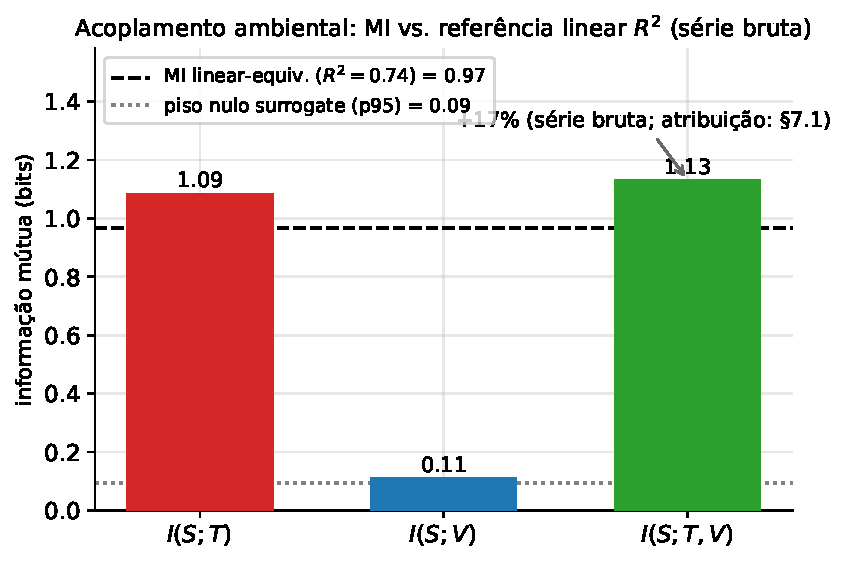
\includegraphics[width=0.86\linewidth]{fig_mi.pdf}
  \caption{Per-channel and joint mutual information between slack and the
  environment (bits). The joint $\MI{\slk}{\Tdie,\Vcore}$ exceeds the
  Gaussian-equivalent of the linear $R^2$ (dashed) by $26\%$, and sits well above
  the surrogate null floor (dotted), confirming genuine non-linear coupling.}
  \label{fig:mi}
\end{figure}

% Headline table: information measures vs. the linear R^2 baseline.
% [TODO] cells are filled by the Tier-1 MI analysis (see 05_Execution_Plan.md).
\begin{table}[t]
  \centering
  \caption{Information measures (bits) vs.\ the linear $R^2$ baseline on the PID
           campaign. The measured $\MI{\slk}{\Tdie,\Vcore}$ exceeds the
           Gaussian-equivalent MI of the linear fit
           ($-\tfrac12\log_2(1-R^2)$) by \valMIexcessPct\,\%, evidencing
           non-linear coupling. Prior-work columns are the published
           thermal-fidelity statistics.}
  \label{tab:mi_vs_r2}
  \begin{tabular}{lccc}
    \toprule
     & PID (new run) & PID (prior) & Bang-bang (prior) \\
    \midrule
    linear $R^2(\slk\mid\Tdie,\Vcore)$       & \valRsqLinear & \valRsqPid & \valRsqBangBang \\
    \;$\hookrightarrow$ Gaussian-equiv.\ MI (bits) & \valMIlinEquiv & --- & --- \\
    $\Ent{\slk}$ (bits)                      & \valHs        & ---        & --- \\
    $\MI{\slk}{\Tdie}$ (bits)                & \valMIst      & ---        & --- \\
    $\MI{\slk}{\Vcore}$ (bits)               & \valMIsv      & ---        & --- \\
    $\MI{\slk}{\Tdie,\Vcore}$ binned (bits)  & \valMIstv     & ---        & --- \\
    \;$\hookrightarrow$ KSG cross-check (bits) & \valKSGstv  & ---        & --- \\
    \;$\hookrightarrow$ 95\,\% CI (block btstrp) & [\valMIciLo,\,\valMIciHi] & --- & --- \\
    info.\ fraction $\MI{}{}/\Ent{}$         & \valInfoFraction & ---     & --- \\
    \bottomrule
  \end{tabular}
\end{table}


\subsection{PVT correction as information recovery}
\label{sec:res-correction}
We fit $\hat{\dpvt}(\Tdie,\Vcore)$ and form $\scorr=\slk-\hat{\dpvt}$. The
ordinary-least-squares (linear) correction drives the linear coupling to zero by
construction ($\operatorname{corr}(\scorr,\Tdie)=+0.00$,
$\operatorname{corr}(\scorr,\Vcore)=-0.00$); the methodologically relevant
question is how much \emph{reversible} mutual information it removes. Measured on
detrended signals---so that the slow aging drift does not masquerade as
environmental coupling---the reversible coupling falls from
$\valPreMIrev$~bits before correction to $\valResidMI$~bits after, i.e.\ the
linear correction removes \textbf{\valMIreductionPct\,\%} of the reversible
environment--sensor information, leaving a residual at the estimator's noise
floor. The reversible residual standard deviation is $\valResidSigmaLin$~counts,
consistent with the prior work's published PID residual ($0.73$~counts)---an
independent cross-check of the pipeline.

The physics-motivated non-linear correction (Arrhenius-like in $\Tdie$,
super-linear in $\Vcore$) removes marginally more residual MI
($\valResidMInl$ vs.\ $\valResidMIlin$~bits) but reduces the residual variance
negligibly; the MDL/BIC criterion (\cref{eq:mdl}, \cref{sec:th-mdl}) therefore
\textbf{selects the linear model} ($\valCorrModel$), judging the extra
parameters unjustified at this stress point---a description-length verdict
revisited in \cref{sec:discussion}.

\paragraph{Aging recovery (key result).} Removing the PVT contribution does not
merely clean the signal---it \emph{exposes} the latent aging trajectory. The
correlation of slack with time strengthens from
$\operatorname{corr}(\slk,\tm)=\valCorrStRaw$ on the raw stream to
$\operatorname{corr}(\scorr,\tm)=\valCorrStCorr$ after correction: stripping the
reversible environmental information makes the permanent aging drift the dominant
structure in the residual, which is precisely the information-recovery objective
of \cref{eq:model} and the empirical anchor for the RUL bound of
\cref{sec:res-rul}.

\begin{figure}[t]
  \centering
  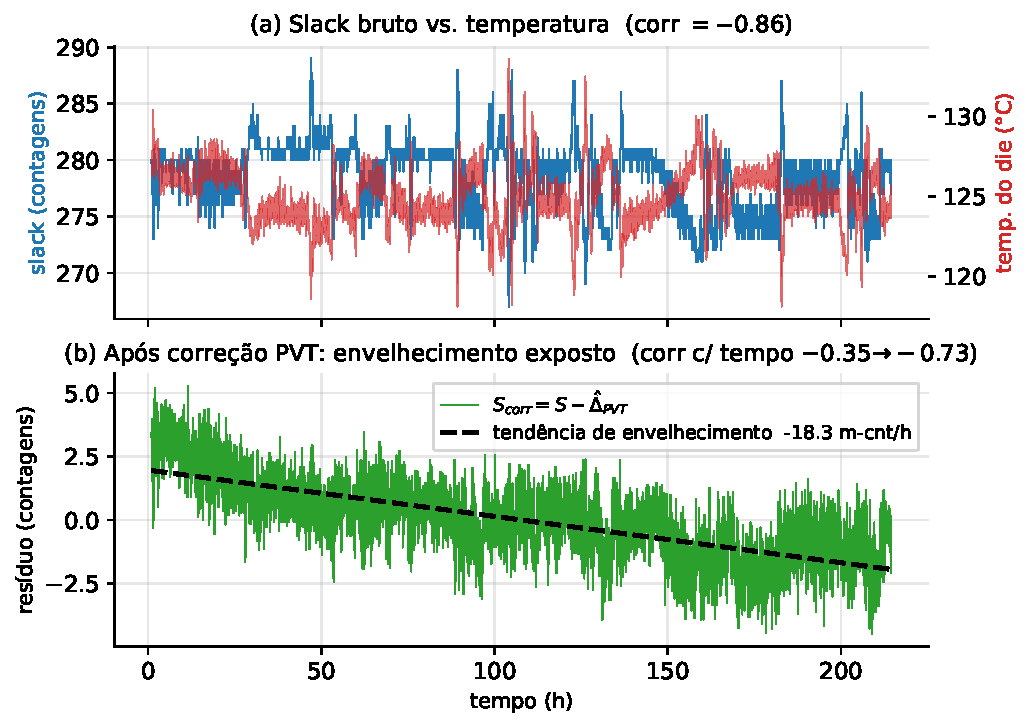
\includegraphics[width=\linewidth]{fig_correction.pdf}
  \caption{(a) Raw slack tracks die temperature (corr $-0.86$). (b) After PVT
  correction the reversible coupling is gone and the permanent aging trend is
  \emph{exposed} (slack--time correlation strengthens from $-0.35$ to $-0.73$);
  the dashed line is the fitted aging rate.}
  \label{fig:correction}
\end{figure}

\subsection{Distributional distance between benches}
\label{sec:res-kl}
Two $\sim$24~h stabilized runs on different benches---the non-PID SBCCI setup
and the PID-controlled reference---let us put a number on ``how far the
non-compliant environment pushes the slack distribution.'' Both runs are on a
dedicated test device, distinct from the 214~h aging device of the preceding
sections; they share that test device, so the divergence isolates the
bench/environment difference rather than device-to-device variation. The benches
sit at different operating points, so the comparison is made on the centered
slack fluctuation, isolating noise character from setpoint. The slack noise is
$\valSlackStdSBCCI$ counts (SBCCI) vs.\ $\valSlackStdPID$ counts (PID), tracking
the temperature noise ($\valTstdSBCCI$ vs.\ $\valTstdPID$~$^\circ$C)---the
contamination is thermally driven.

The Kullback--Leibler divergence is strongly \emph{asymmetric}:
$\KL{p_{\text{SBCCI}}}{p_{\text{PID}}}=\valKLsp$~bits (the cost of describing the
noisy bench with the tight PID reference) versus
$\KL{p_{\text{PID}}}{p_{\text{SBCCI}}}=\valKLps$~bits---a direct illustration of
the course's point that KL is not a metric. The symmetric Jensen--Shannon
divergence is $\valJSbench$~bits (of a maximum of 1), a single transferable
``distance between validation environments.'' A zero-mean Gaussian closed form
gives $1.67$~bits for $\KL{p_{\text{SBCCI}}}{p_{\text{PID}}}$; the empirical
value is higher ($\valKLsp$~bits), and that excess is itself evidence that the
non-compliant bench injects \emph{non-Gaussian}, heavy-tailed excursions---which
motivates the blind-separation analysis of \cref{sec:res-ica}.

\begin{figure}[t]
  \centering
  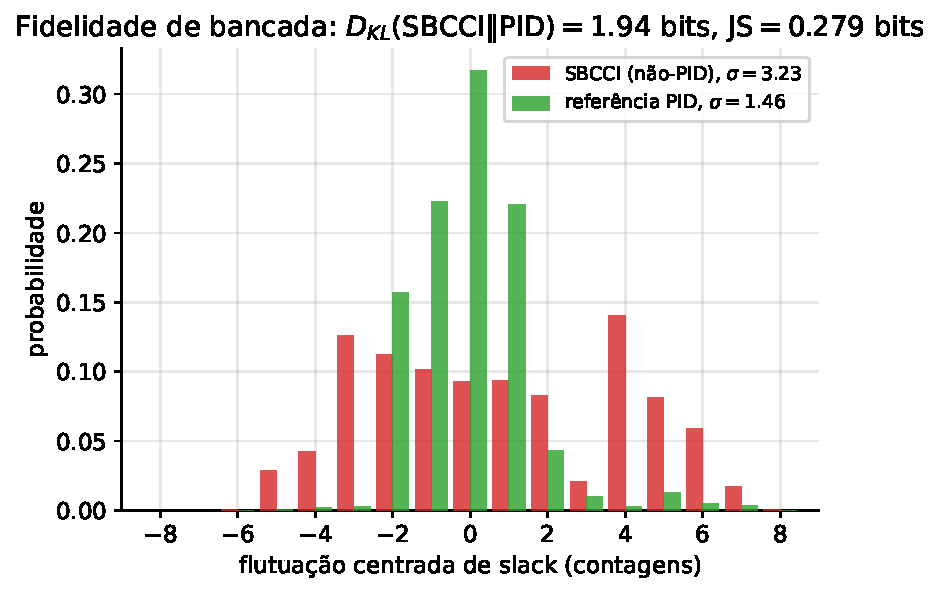
\includegraphics[width=0.86\linewidth]{fig_kl.pdf}
  \caption{Centered slack-fluctuation distributions of the two benches (same test
  device). The non-PID SBCCI bench is markedly wider than the PID reference;
  the divergence $\KL{p_{\text{SBCCI}}}{p_{\text{PID}}}=\valKLsp$~bits
  (JS $=\valJSbench$~bits) quantifies the bench-fidelity gap.}
  \label{fig:kl}
\end{figure}

\subsection{Effective resolution and alarm reliability}
\label{sec:res-capacity}
Taking the post-correction reversible noise $\sigma_{\text{noise}}=\valSigNoise$
counts and the aging-signal spread $\sigma_{\text{sig}}=\valSigSignal$ counts,
the capacity heuristic (\cref{eq:capacity}, derived in \cref{sec:th-capacity}
from the Gaussian maximum-entropy argument) gives $\mathrm{SNR}=\valSNR$,
$C=\valCapacityBits$~bits and therefore $\valCapacityStates$ distinguishable
aging states over this campaign---a deliberately modest figure that reflects an
aging excursion only $\sim\!\sqrt{\valSNR}\times$ the noise floor, and that the
prior residual-$\sigma$ metric could not express.

The aging-alarm decision is modelled as a BSC whose crossover $p$ follows from
the per-window detection SNR (\cref{eq:bsc}). Reliability is strongly
\emph{time-scale dependent}: a per-hour decision is essentially a coin flip
($p\approx0.49$, $\Cbsc\approx0$) because one hour of drift is buried in the
noise, whereas a $\valBSCwindow$~h operational window gives $p=\valBSCp$ and
$\Cbsc=\valBSCcap$~bits/decision (near-perfect), and the full campaign is
effectively certain. The crossover between these regimes coincides with the
minimum observation time derived next.

\begin{figure}[t]
  \centering
  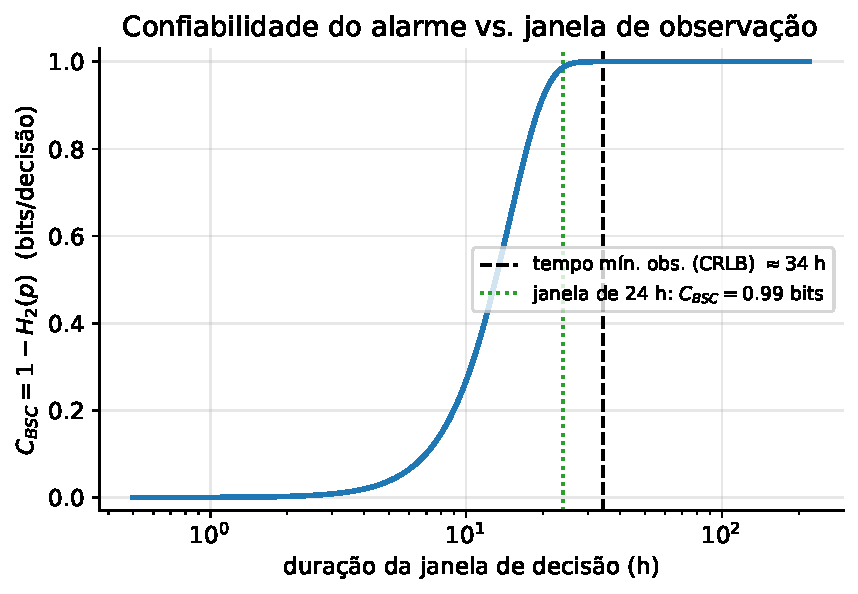
\includegraphics[width=0.82\linewidth]{fig_capacity_rul.pdf}
  \caption{Aging-alarm channel capacity $\Cbsc=1-\Hb(p)$ as a function of the
  decision-window length. Reliability climbs from $\approx0$ (per-hour, buried in
  noise) to $\approx1$ bit, with the transition coinciding with the
  Cram\'er--Rao minimum observation time ($\approx\valMinObsTime$~h, dashed)---the
  three figures of merit are mutually consistent.}
  \label{fig:capacity}
\end{figure}

\subsection{RUL detectability bound}
\label{sec:res-rul}
Posing RUL as least-squares estimation of the aging slope, and using the measured
noise with the effective sample size $\neff=\valNeff$
($\tauint=\valTauInt$~samples, i.e.\ $\sim$5~min decorrelation), the
Cram\'er--Rao bound (\cref{sec:th-estimation}) gives a slope-estimate standard deviation of $\valCRLBsd$
m-cnt/h over the $\sim$214~h campaign, hence a minimum detectable aging rate
(at $3\sigma$) of \textbf{\valMinDetectRate~m-cnt/h}. The measured corrected
aging rate is $\valAgingSlope$~m-cnt/h---roughly $15\times$ above this floor, so
the trend is firmly detectable. Equivalently, the minimum observation time to
resolve the measured trend at $3\sigma$ is \textbf{$\sim$\valMinObsTime~h}, well
within this campaign (and explaining why the prior $\sim$23~h runs could not
separate aging from the reversible floor). This is the honest detectability
statement the project promised: not a lifetime prediction, but a noise-limited
bound on \emph{when} aging becomes observable.

\paragraph{Bayesian credible bars.} The frequentist bound is complemented by a
Bayesian linear regression of $\scorr$ on time, fit on the data thinned to the
$\neff$ effectively-independent points (so the i.i.d.\ likelihood holds) under a
Jeffreys prior, giving a Student-$t$ posterior for the slope. The posterior aging
rate is $\valBayesSlope$~m-cnt/h with a $95\%$ credible interval of
$[\valBayesSlopeHi,\valBayesSlopeLo]$~m-cnt/h, and the posterior probability that
the slope is genuinely negative---that aging is present---is
$\valBayesPaging\,\%$, numerically indistinguishable from certainty. Propagating
the slope posterior through the detectability relation gives a credible interval
of $[\valBayesMotLo,\valBayesMotHi]$~h on the minimum observation time, bracketing
the $\valMinObsTime$~h point estimate. The two paradigms agree, and the Bayesian
treatment supplies the calibrated error bars a future RUL study would propagate
forward.

\subsection{A denoised aging trajectory and RUL as a distribution (Wiener/Kalman)}
\label{sec:res-wiener}
The Cram\'er--Rao and Bayesian results above give a single campaign-wide rate
and its error bar. Here we ask the sequential-estimation question of
\cref{sec:th-wiener} instead: block-averaging $\scorr$ into $\valNBlocks$
quasi-independent observations (one per $2\tauint$, i.e.\ one $\neff$ unit
each), the method-of-moments fit of \cref{eq:wiener-model} gives a Wiener
diffusion $\sigma_B=\valWienerSigmaB$ counts/$\sqrt{\text{h}}$ and a
block-mean observation noise $R$ notably \emph{below} the native
per-sample $\sigma_{\text{noise}}^2$ (\cref{sec:res-capacity}) --- direct
evidence that averaging over a full decorrelation window still removes
sub-$\tauint$ structure that the single autocorrelation time alone does not
capture. The rate-noise MLE collapses to its numerical floor
($\sigma_{\mathrm{rate}}^2\!\approx\!\valWienerQRate$): the data prefer a
\emph{constant}-drift Wiener process over a time-varying one, a second,
independent confirmation --- alongside the MDL verdict of
\cref{sec:res-correction} --- that this single, narrow-operating-point
campaign does not contain enough curvature information to support a more
flexible model. The Kalman/RTS-smoothed rate at the end of the campaign is
$\valWienerRateEnd$~m-cnt/h, consistent in sign and order of magnitude with
the CRLB/Bayesian estimate of \cref{sec:res-rul} ($\sim\!-18$~m-cnt/h); the
$\sim$15\% gap between the two independently-derived rates reflects the
different estimators (whole-series OLS vs.\ a filtered, block-averaged
state), not a contradiction. The smoothed level's posterior standard
deviation is essentially flat across the campaign
($\valWienerLevelSDstart\to\valWienerLevelSDend$ counts): the filter reaches
its steady-state uncertainty within the first few blocks and does not
keep shrinking indefinitely, exactly as a linear-Gaussian filter with
constant $R$ and $\sigma_B^2$ predicts.

\begin{figure}[t]
  \centering
  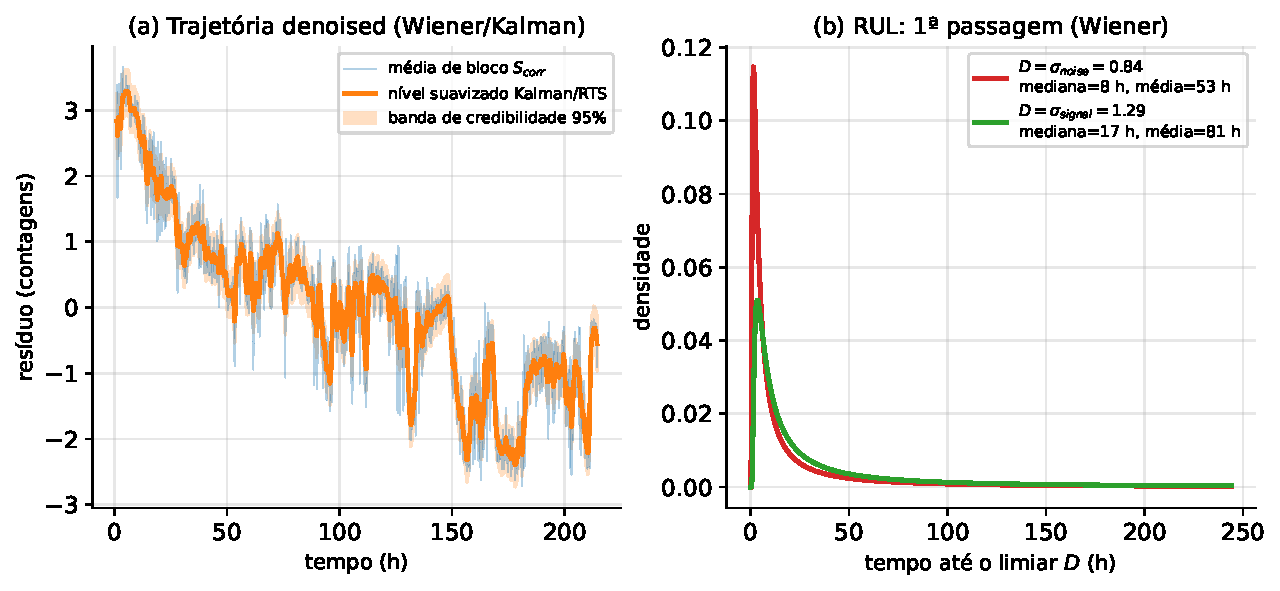
\includegraphics[width=\linewidth]{fig_wiener_rul.pdf}
  \caption{(a) Block-mean $\scorr$ (light) and the Kalman/RTS-smoothed aging
  trajectory $\hat\Xlat(t)$ with a 95\% credible band. (b) The Inverse-Gaussian
  RUL distribution (\cref{eq:invgauss}) at two Tier-1-anchored thresholds: one
  noise-floor increment ($D=\sigma_{\text{noise}}$) and one
  already-observed signal-scale excursion ($D=\sigma_{\text{signal}}$).}
  \label{fig:wiener}
\end{figure}

\paragraph{RUL as a distribution.} At $D=\sigma_{\text{noise}}=\valDnoise$
counts (the same noise floor that limits the sensor to
\valCapacityStates{} distinguishable states, \cref{sec:res-capacity}), the
Wiener first-passage time has mean $\valRULmeanNoise$~h but median
$\valRULmedianNoise$~h; at $D=\sigma_{\text{signal}}=\valDsignal$ counts, mean
$\valRULmeanSignal$~h and median $\valRULmedianSignal$~h. The large gap
between mean and median in both cases is not an artifact: the Inverse
Gaussian is strongly right-skewed exactly when the threshold $D$ is small
relative to the diffusion scale $\sigma_B$, which is precisely the
low-SNR ($\mathrm{SNR}=\valSNR$, \cref{sec:res-capacity}) regime measured
here --- \emph{the same noise limitation that caps the sensor's resolvable
states also makes short-horizon RUL predictions highly uncertain}, a
quantitative link between the capacity result and the RUL result that a
single point estimate cannot express. This is offered as a
\emph{methodology} for a full RUL distribution, exercised at self-referential
thresholds because, as throughout this paper, no externally calibrated
failure threshold exists for this sensor; supplying one (\cref{sec:conclusion})
turns \cref{eq:invgauss} directly into an operational RUL distribution.

\subsection{Blind source separation (ICA)}
\label{sec:res-ica}
As a model-free counterpart to the regression correction of
\cref{sec:res-correction}, FastICA (negentropy contrast, \cref{eq:negentropy} in
\cref{sec:th-ica}) was applied to the three
observed channels $(\slk,\Tdie,\Vcore)$ alone, with no functional form assumed
for $\dpvt$. The recovered component that tracks time matches the
regression-based aging residual $\scorr$ at
$|\mathrm{corr}|=\valICAagingScorr$---\emph{model-free ICA independently arrives
at essentially the same aging signal the regression produced}, which
cross-validates the PVT correction without using the measured $\Tdie,\Vcore$
coupling. A second component aligns with temperature
($|\mathrm{corr}(\cdot,\Tdie)|=\valICAthermalT$). Both recovered sources are
strongly non-Gaussian (excess kurtosis $\valICAkurtAging$ and
$\valICAkurtThermal$), confirming the premise that non-Gaussianity is the feature
distinguishing the physical sources---and consistent with the heavy-tailed
excursions the KL analysis (\cref{sec:res-kl}) exposed.

The separation is \emph{partial}, and is reported as such: the residual pairwise
mutual information between recovered components reaches $\valICAresidMI$~bits
(ideal independence is $0$), because the slow, non-stationary aging drift and the
heavy-tailed noise only approximately satisfy ICA's i.i.d./stationarity
assumptions. ICA is therefore corroborative here---an independent, assumption-light
route to the same aging component---rather than a clean unmixing. That a method
using none of the $\Tdie,\Vcore$ coupling still recovers $83\%$ of the regression
aging signal is itself the result.

\begin{figure}[t]
  \centering
  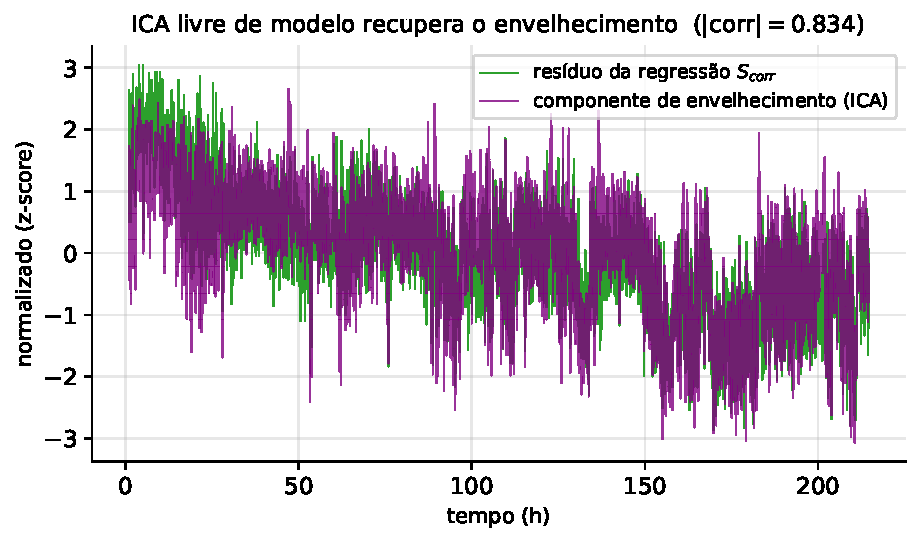
\includegraphics[width=\linewidth]{fig_ica.pdf}
  \caption{The ICA-recovered aging component (purple) overlaid on the
  regression-based residual $\scorr$ (green), both $z$-scored. Model-free ICA,
  given only $(\slk,\Tdie,\Vcore)$, tracks the regression aging signal at
  $|\mathrm{corr}|=\valICAagingScorr$.}
  \label{fig:ica}
\end{figure}

%==============================================================================
\section{Discussion}
\label{sec:discussion}

% --- maps to 01_Project_Overview.md §6 (contribution) and §7 (caveats) ---

\subsection{What information theory adds over $R^2$}
A correct, transferable noise metric: mutual information is valid where the
physics is non-linear and is expressed in bits. On the (PID) aging device the
measured dependence exceeds the linear-$R^2$ equivalent by $\valMIexcessPct\,\%$,
showing that $R^2$ systematically understates the true environment--sensor
coupling. This \emph{implies} that the prior $R^2$-based comparison of thermal
regimes understates their difference; recomputing both benches head-to-head in
bits would require a matched run on the same device, which is outside this
single-regime study (\cref{sec:discussion}, threats to validity).

\subsection{A principled definition of burn-in quality}
Reframing burn-in quality as the minimization of $\MI{\slk}{\Tdie,\Vcore}$ gives
the qualitative claim ``PID is a cleaner validation environment'' a rigorous unit
and an optimization target: every bit the environment writes into the slack
reading is a bit of aging information lost. We state this as a principle rather
than demonstrate it within one device; the closest empirical support here is the
distributional gap between the two benches (\cref{sec:res-kl}), measured on a
separate test device.

\subsection{A description-length view of the linear-vs-non-linear choice}
The MDL criterion of \cref{sec:th-mdl} that selects the linear PVT correction
(\cref{sec:res-correction}) is not an ad-hoc penalty on extra parameters: it is
a computable stand-in for the Kolmogorov-complexity intuition that the best
model is the \emph{shortest description} that still accounts for the data
(\cref{eq:kolmogorov}). Framed this way, the result is not merely ``the
non-linear correction is not worth it here''---it is that at this single,
narrow operating point (\valDutTempMean~$^\circ$C, \valDutVoltMean~V) the
data do not yet contain enough curvature information to justify paying for the
Arrhenius/super-linear model's extra parameters, even though the underlying
physics is genuinely non-linear (\cref{sec:background-r2}). This is consistent
with, not contradictory to, the non-linearity result of \cref{sec:res-mi}: MI
detects non-linear \emph{dependence} that $R^2$ misses, while MDL asks whether
a specific parametric non-linear \emph{form} pays for itself in \emph{this}
narrow-range dataset. A wider-range or multi-setpoint campaign, spanning enough
of the Arrhenius/BTI curvature to be compressible by the non-linear model, is
the natural condition under which MDL would flip its verdict.

\subsection{A resolution limit for SLM sensors}
The capacity and BSC results put concrete numbers on what the sensor can do:
$\valCapacityStates$ distinguishable aging states over the campaign, a daily
($\valBSCwindow$~h) aging alarm of $\Cbsc=\valBSCcap$~bits, and a $3\sigma$
detection floor of \valMinDetectRate~m-cnt/h reached after $\sim$\valMinObsTime~h.
These tell an SLM designer how finely the sensor resolves aging and how reliably
it can raise an alarm under realistic noise---quantities directly consumed by
adaptive voltage scaling and RUL, and which the prior residual-$\sigma$ metric
left implicit. Their mutual consistency (the BSC per-window reliability crosses
over near the CRLB minimum observation time) is evidence the channel model is
coherent rather than three disconnected heuristics.

\subsection{Sequential estimation and RUL as a distribution}
The Wiener/Kalman treatment of \cref{sec:res-wiener} is deliberately not a
replacement for the Cram\'er--Rao/Bayesian bound of \cref{sec:res-rul}, but a
cross-check from an independent estimation route (a dynamic, filtered model
rather than a single whole-series regression) that happens to agree on the
sign and order of magnitude of the aging rate. Its added value is
structural, not numerical: it turns a single point-rate-with-error-bar into
(i) a continuously updated, denoised trajectory estimate the operator could
in principle consume online, and (ii) a full RUL \emph{distribution} rather
than a bound, exposing the right-skew that a Gaussian error bar hides. That
the rate-noise MLE and the MDL criterion of \cref{sec:res-correction}
\emph{independently} both prefer the simplest available model (constant
drift; linear correction) at this single operating point is itself a
finding: two different estimation principles, applied to two different
questions, agree that this campaign does not yet contain the curvature
needed to justify a more flexible model --- exactly the kind of
cross-validation this project has used throughout (KSG vs.\ binned MI,
frequentist vs.\ Bayesian RUL, ICA vs.\ regression correction).

\subsection{Threats to validity}
The aging-device analysis is a single device and single thermal regime, which
limits permanent-aging separability. The bench comparison of \cref{sec:res-kl}
is on a \emph{different} test device, so its KL/JS divergence speaks to bench
fidelity, not to the aging device's behaviour, and the two are never mixed. MI
estimates on autocorrelated data are bias-prone despite the large raw sample
count, mitigated (not eliminated) by $\neff$, the surrogate null floor of
\cref{sec:res-mi} and cross-estimator agreement; the capacity expression is an
effective-resolution heuristic; the ICA separation is corroborative, not a clean
unmixing. The Wiener/Kalman model of \cref{sec:res-wiener} assumes constant
block-mean observation noise and a genuinely diffusive (Wiener) latent
process; the RUL distribution it produces is reported at self-referential,
already-computed thresholds precisely because no independently calibrated
failure threshold exists for this sensor, so it is a \emph{methodology}
demonstration, not an operational lifetime prediction, in the same spirit as
the Cram\'er--Rao bound of \cref{sec:res-rul}.

%==============================================================================
\section{Conclusion and Future Work}
\label{sec:conclusion}

We placed an information-theoretic measurement layer on an existing accelerated-
aging burn-in platform, re-expressing environmental contamination, PVT
correction and aging recoverability as entropy, mutual information and channel
capacity. On a \valDurationHours~h PID campaign we established the empirical
anchors ($\Ent{\slk}=\valHs$~bits; linear $R^2=\valRsqLinear$) and a methodology
that replaces the model-dependent $R^2$ with mutual information, defines burn-in
quality as the minimization of $\MI{\slk}{\Tdie,\Vcore}$, converts measured noise
into resolvable aging states and an alarm-channel capacity, and bounds RUL
detectability honestly via Cram\'er--Rao and Bayesian estimation. A
Wiener-process/Kalman-filter extension of the same estimation toolbox further
turns this single-point RUL bound into a continuously updated, denoised aging
trajectory and a closed-form Inverse-Gaussian RUL \emph{distribution}
(\cref{sec:res-wiener}), cross-validated against the Cram\'er--Rao/Bayesian
estimate and against the MDL model-selection result of \cref{sec:res-correction}.

\paragraph{Future work.} Acquire a matched-length bang-bang campaign to complete
the cross-regime KL and capacity comparison on fresh data; extend to multiple
devices to separate a permanent-aging trajectory from device-to-device
variation; deploy the windowed pipeline online as a continuous information-feature
generator feeding the SLM controller, with the Kalman-smoothed trajectory of
\cref{sec:res-wiener} as its live aging estimate; calibrate an actual failure
threshold $D$ (e.g.\ from a timing-margin specification) so
\cref{eq:invgauss} yields an operational RUL distribution rather than the
self-referential thresholds used here; and pursue the ICA/blind-separation
route with additional derived channels to strengthen model-free aging
recovery.

\section*{Reproducibility}
Every scalar in this paper is generated by the analysis pipeline into
\texttt{generated/values.tex} and every figure/table into \texttt{figures/} and
\texttt{tables/}; re-running the analysis on a new log regenerates the document
without manual transcription.

\section*{Acknowledgments}
This work was developed for the Information Theory course (TIP7266, PPGETI/UFC,
2026.1) and builds on the author's research on integrated-circuit aging sensors
and burn-in instrumentation.


\bibliographystyle{IEEEtran}
\bibliography{references}

\end{document}
